% !TEX root = report.tex

\chapter{Strategy}
\label{chap:strategy}

In this chapter we discuss our decisions for the strategy used by \massexpand{}. The strategy of a bot is the most important part of the bot, as not only does it involve the overall structure of the bot, but also how it makes decisions.

The \emph{output} of the strategy, the decisions and how it plays, is in essence a \emph{behaviour}. Based on the type of decisions, the behaviour of the bot changes. As for the \emph{input} that induces the decisions, we view two different possibilities: perception and internal. The former is information observed or input by the player or the game, whereas the latter comes from internal variables or the 'mood' of the bot.

We call decisions based purely on perception \emph{reactive}, and decisions only based on internal variables \emph{proactive}. For example, when a bot makes a decision based on the observation of five enemy units, it makes a reactive decision. And if the bot makes a decision when 'two minutes have passed', it makes a proactive one. It is also possible to make decisions based on both types of input, for example the decision to make additional units when enemy units are observed and when the bot is in a 'defensive mood'.

Each decision made by the bot (and player) has an impact on the game. When a bot sends units to the enemy, the game changes, as units may get damaged and lost. The player that still has  units left over, while the other does not, wins the game in StarCraft. However, it is rarely the case that all of one's units are lost in a single fight. Understanding the impact of small fights is not an easy thing to do. Even if we lose every unit in some fight, we may still have succeeded in doing enough damage that eventually would lead to winning the game.

For bots, matters are even more complicated as winning may not always be its objective. Although humans usually seek to win, bots may be designed to entertain the player. The focus is then to play interesting moves and make fights interesting for the human player.


Naturally, understanding the game and making correct decisions to accomplish an objective are the most difficult concepts intrinsic to the game. In a strategy game like StarCraft, there are many factors to be considered: the units that fight one another, the armor rate and armor type of a unit, the temporary abilities affecting the units, commands being issued, and so on. 

The same holds for most other strategy games. As a result, most developers of such games do not consider to design elaborate AI bots. Rather, the bots often follow a simple script that is executed regardless of the opponents' moves. Such a design makes the bot's decisions quite predictable, resulting in human players easily finding an optimal strategy against the bot. When an optimal strategy against a predictably playing bot is found, the 'replay value' of playing against that bot decreases.

Often, the scripts used by AI bots are not very adaptive. Instead, the scripts are run using a set of timers or preset conditions. Even the hard (highest difficulty) AI that is sometimes implemented in games use a similar method. Extra difficulty is usually achieved by cheating: the bots are given extra resources, free units, little to no time required to build units, full observability (when there is a fog of war), and so on.



%The hardest part of the game is to understand what decisions are good and which are bad. This notion depends on what our ulterior objective is. Most often this is just 'winning the game', or in the case of a bot 'entertaining the player' by creating interesting gameplay. 

%For strategy games, such as StarCraft, we find that bots tend to just follow a simple script. As a result, the bot plays very similarly every game, regardless of the opponent. This makes the bot predictive, making it possible for the player to easily find a winning strategy. Another issue is that these bots tend to have little to no reactive behaviour. Thus, when a player pursuits a certain strategy, the bot does not dynamically adapt at all. Arguably, this does not create much extra value to the game.


%Even the so-called 'hard AI' implemented in games for bots follow a similar paradigm. The extra difficulty is then often that the bot are provided with a lot of resources, allowing it to build whatever it wants. Furthermore, bots are often given full observability of the game. Consequently, bots send full attack forces to secret bases of the player. So rather than the bot being better at the game, it just cheats even more. All these things make playing against bots, for a human, rather uninteresting. 

When entering a competition, the goal is usually to win. Despite our participation in the AIIDE2010, we did not focus on creating a winning bot. Instead, we focused on creating a bot that provides interesting gameplay that is not completely predictive and adapts to the player, without cheating. Creating a bot capable of winning the tournament quickly turned out to be out of reach, because of the time and knowledge needed. The problem space was simply too large, as will be explained later in this chapter. Therefore, we directed our efforts towards creating a bot that could play the game 'well-enough', adaptively and autonomously.

Creating a strategy for StarCraft is a very difficult problem. The bot has to consider every aspect of the game: harvesting resources, training the right units, building the right structures at the proper locations, adapt automatically to the opponent, placing units at the right location on the map to anticipate enemy attacks or prepare for an attack of its own, attack enemy units at the right place and time with minimal losses, scouting locations for information about the enemy, and so on. Generally, the whole problem is that of properly assigning units to go to certain locations and have them attack enemy units, and getting enough resources to train enough units.

\begin{figure}
\centering
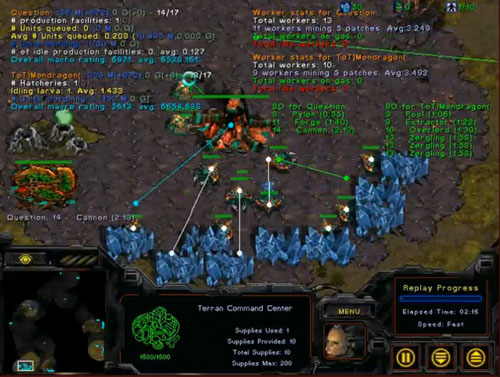
\includegraphics[scale=0.6]{bwapi.jpg}
\caption{\label{fig:bwapi} A replay of an AI bot playing StarCraft. The textual information on the screen is for debugging purposes only, and is not used by the bot itself.}
\end{figure}

% **** dits eigenlijk geen ai bot, maar gewoon een replay

For the remainder of this chapter, we first sketch some general appoaches and techniques that are possible to make bots play, in section \ref{sec:techniques}. After describing the general approach for the design of the bot, we explain the race selection for our bot in section \ref{strategy:race}. Then, we go into more detail on how to build, train and upgrade units in section \ref{strategy:but}, how we organize units on a strategic level to attack and defend in section \ref{strategy:macro}, and how to control units individually and make appropriate decisions in section \ref{strategy:micro}. We do not describe the code itself, but rather the abstract choices relevant for the strategy of the bot. In the next chapter we go into more detail on the implementation of our bot.


\section{General Approach and AI Techniques}
\label{sec:techniques}

Research in the field of Artificial Intelligence has shown that there are various ways for a computer to play a game. We will name a few and discuss how they work. The choice of technique is important as it guides how we approach the problem of developing a bot, and ulteriorly what information and knowledge we need.


The first technique considered is related to 'board simulation' and 'board evaluation'. The term 'board' comes from board games, but in computer games generally refers to the game state. The idea is to first start with the current board and then, by considering various possible decisions, simulate new hypothetical boards. These hypothetical boards can be viewed as a possible future on the current board when certain decisions are made. We can repeatedly do this on the newly simulated boards, to simulate boards 'deeper'. The depth of this simulation is commonly referred to as \emph{ply}, e.g. one decision deep is a 1 ply simulated board, and three decisions is 3 ply.

After a number of boards are simulated, we can \emph{evaluate} them on how 'beneficial' they are for the bot. Then, by tracing back what decisions lead to the most beneficial board, we can guide our decision process. This tracing back mechanism can be viewed as searching through a decision tree.

Unfortunately, this technique assumes three important things. First, it assumes that we can accurately simulate boards. This requires us to know how the board will change after a decision. The second assumption is that we have a function that can evaluate precisely how beneficial the board is. The third assumption is that the boards themselves can be computed in a reasonable amount of time.

With our knowledge of StarCraft, we cannot fulfill the first two assumptions. The first assumption requires us to fully understand the game engine and how units interact with one another. Not only does such an understanding take an immense amount of time, this understanding would also have to be implemented in the bot in the form of the ability to 'recreate' entire games internally. The second assumption requires us to have a reasonable understanding of the gameplay, strategies and tactics. As explained earlier, we do not have the necessary knowledge. In fact, such an understanding is precisely what professional players of StarCraft try to achieve over many years. Even if we do have some idea of what is a good move and what is not, we will have to quantify these moves somehow to allow for a clear selection of the 'best board'.

The third assumption is of a more computational nature, which depends on our choice of algorithm and how boards are simulated. Although there are many choices, we believe that without good knowledge of the game, it is hard to avoid simulating many boards. In theory, it is perfectly feasible to simulate boards. However, in practice, the simulation of boards quickly becomes unpractical.

For example, an average game of StarCraft tends to have between 30 to 150 units, and on average a unit has 6 actions.\footnote{This number of average actions per unit does not take into account that some actions may also be pointed at any unit or area in a range of the unit, such as spells of caster units.} Let us assume that at average games have an average of 80 units during the game. Then, if we consider that each unit can get issued a command per timestep of the game, we have $6^{80} \approx 1.8.10^{62}$ hypothetical boards at 1 ply deep. This is a very large number for only a very low ply and indicates that the computation of boards is very expensive.

An alternative technique is to \emph{learn} which decisions are good. This approach has some similarities to the previous technique. As the learning system interacts with the board, it makes random decisions and tries to find a pattern in the decisions it made and the consequent of these decisions, such as a win or loss. From the pattern found, it can conclude what decisions are good in which boards. Thus, the similarity is that it also involves 'simulation' and 'evaluation' of a board. The foremost difference is that this approach tries to learn a \emph{function} that chooses good decisions based on experience beforehand, whereas the previous approach simulates hypothetical future boards while playing and chooses a decision.

The problem with this technique is that it requires a lot of time. Each board must be reviewed several times to learn what decisions are good or bad. Also, there are many different boards possible in a game of StarCraft. Even if we only consider the same number of average units before (80), they can all be placed in numerous ways, each placement resulting in a totally different board. Even if we assume that we can come across every board, we still need to find a learning algorithm powerful enough to find a pattern in all the information. We do not know any algorithm that can take into account all possible boards, dependencies on the past, unknown information of the opponent (as there is partial observability), actions available, and so on. The development of such an algorithm requires a lot of more knowledge on how systems learn such complex problems.

Another technique that can be considered is an algorithm that learns from a human player \emph{showing} how to play. As the human player plays the game and makes decisions, the algorithm assumes that the player makes good decisions and tries to memorize them. This is an interesting approach, but it assumes the availability of a player who is objectively regarded as an expertl. The alternative is to use \emph{replays} of games. Replays are widely available, but still leaves us with one other problem. Even if we do memorize what decisions are good, the bot that we develop may often find itself in a totally new situation for which it does not know what to do. Finally, it is not always easy to see whether decisions were actually good.

The consideration of different techniques gave us some ideas for creating our own AI. There are several websites and forums dedicated to strategy discussion for StarCraft, from low-scale tactics to overall orders in which buildings should be built. We found most of them to be quite high level, but they do describe in a lot of detail how units should move and attack. If each unit does exactly what it should do, the result should be a overall well-playing bot.

This insight gave us the idea to adopt an approach of \emph{self-organisation}, where units interact as if there are single-minded. Simply put, we expect emergence to occur from all the simple interactions of individual units. This gives two interesting benefits: first we do not need to consider to compute a whole plan for every unit, but instead can focus on how an unit by itself should work; and secondly because there is no overall plan, and units adopt by themselves, we allow for adaptivity to the opponent without writing complete explicit scripts on what to do.

Therefore, we decided to adopt this approach of controlling units individually by writing behaviour for each type of unit separately. The only necessity then is a description of \emph{appropriate behaviour}, which is luckily prevalent on internet websites and forums.

StarCraft, however, brings some additional challenges to coding it in an self-organising way. Namely, the resources available are attached to a person instead of to units. To prevent scenarios from occuring where multiple units decide 'it is good' to build new units and use resources, we must find some solutions that do not necessarily stick to the self-organisation approach.

Another point of consideration is how to let multiple units decide to attack. Consider for instance the case when only a few units decide to attack when the enemy forces are substantially larger, or when a unit decides to attack an enemy unit when it is better to focus its attacks elsewhere. For this, we will consider an approach that forms groups of units, allowing for easy control on a strategic level.

In the following section we describe our choice of the race and sources. In the next sections after that we describe in detail how we decided what is good behaviour, how units are built, and how units work together.

\section{Race Selection and Sources}
\label{strategy:race}
In the game of StarCraft, there are three playable races: the Terran, representing the human, using technology and machinery; the Protoss, an alien humanoid race focusing on energy forces and psychic powers; and the Zerg, an alien race thriving on evolution to get stronger biotics and slash enemies.

For our bot, race selection is important. First, we did not expect have time to create a bot that can play all three races. Each race plays very differently and accounting for that would require an immense amount of time. Second, races require different mechanics and types of AI. Some require a lot of planning on how structures are placed, or how units should fight along each other. We decided to choose the race that is easiest to control from an \emph{emergent} AI perspective.

The Terran focus on using ordinary guns, lasers and cannons. Most of their units have ranged attacks. The training costs of Terran units are relatively balanced, as Terran units fall in between units of the other races regarding their power. The Protoss on the other hand focus more on powerful but expensive units. As a result, Protoss players tend to have fewer units than both Zerg and Terran players. In general, Protoss units also have more special abilities than Zerg and Terran units. The Zerg mostly have fairly bland units with little abilities. Their power comes from their numbers, as Zerg units are very cheap, but also somewhat weak. It is out of the scope of this report to give the complete details of every unit, structure and upgrade.

The three races' units obviously have to be controlled differently, and strategies differ a lot between them. The ways in which the three races build structures are even more different. The Protoss \emph{warp} buildings to the battlefield, requiring only a simple worker unit (a Probe) to mark the location for the building. The Terran require a worker unit (an SCV) to invest time on building the structure. If the worker is interrupted or killed during construction, the structure is left incomplete. Finally, the Zerg have their workers (Drones) \emph{evolve} into the desired buildings. The Drone is lost, but compared to the Terran and Protoss, the Zerg require relatively few buildings.

The structures of both Protoss and Terran need to invest time in training new units. As only one unit per training facility can be trained at a time, players often make many more structures of the same type. This allows more units to be trained at the same time, giving the player the possibility to adapt quickly to new information of the opponent and train a new army more quickly. The Zerg work slightly differently: at short intervals, up to three uncontrollable units called Larva spawn at each of the Zerg player's main structures (Hatcheries and their evolved versions, Lairs and Hives). These Larva can be commanded to evolve into a specific unit, such as a worker or combat unit. Zerg structures do not train units themselves, but allow the Larva to evolve into different types of unit. As a result, each structure is only required once. For a higher unit production rate, Zerg players create more Hatcheries.

Initially, we believed that Terran units were the easiest to control. Because all of their units can shoot from a distance, they are only required to move in the \emph{right direction}, not even having to order them to shoot at enemy units as they do so automatically. However, the management of Terran structures is quite complicated: what structures to build and how many, but also where to place them. We found that there is a whole science behind how buildings should be placed, as they can be of assistance in fights. For instance, Terran buildings can be strategically placed to prevent enemy units from accessing bases. For Protoss, the same holds for the structures, but the combat units themselves have to be moved more delicately, too. 

As for the Zerg, however, structure placement is important too, but slightly easier to manage: Zerg structures are often placed so that there is a lot of space for units to move through. This is because the Zerg player often has large numbers of units. Also, the training of units is very easy for the Zerg, as Larva availability generally is not a problem. Furthermore, the Zerg units are easily steered. Finally, the Zerg seemed to fit the idea of \emph{emergence} wel because of their alien insect theme. Therefore, we decided to create a bot that plays Zerg.

Once we had decided on the race, we tried toobtain good strategies against each kind of opponent. In other words, even though we selected one race that the bot would play, we still had to develop three different AIs, for each possible race the opponent may select. This is because the playstyle of the Zerg substantially differs per enemy race.

For the AI of the Zerg, we used three different types of sources: websites on strategy discussion, feedback and knowledge elicitation from people familiar with the game, and \emph{replay videos} of matches between professional players. From this, we could understand the game, how units can be controlled, various strategies and so on.

%sourcelist***

\section{Spending Resources: Building, Upgrading and Training}
\label{strategy:but}
We first discuss how our agent spends gathered resources. Gathered resources can be spent by either building structures, upgrading abilities and units, and training new units. The mechanic of StarCraft is that resources are bound to a player, rather than a unit or specific area. That means that if resources are collected on one side of the map, we can use the resources instantly at a different location.

In StarCraft, there are two gatherable resources, minerals and vespene gas, and one generated resource, the supply cap. Minerals and vespene as have to be gathered from mineral crystals and vespene geysers respectively. These two resources are necessary to create anything. The supply cap on the other hand is simply a limit on the number of units the player may have. By creating additional racial-dependent units or structures, this limit can be increased. The Zerg increase the supply cap by creating Overlord units. Naturally, any units owned by the player increment the current supply. Once the limit will exceed with a new unit or has been exceeded, the player can not create any new units.

Overall, strategies in StarCraft revolve around gathering resources and destroying the opponent's resources. Players that have little or no resources left tend to lose the game, because they can no longer create units. The same holds for the supply cap: by destroying units increasing a player's supply cap, the opponent cannot reinforce his army and may quickly be overwhelmed.

For our bot that plays the Zerg race, we have the benefit that almost all structures only have to be built once. This means that we eventually do not have to consider building anymore and the bot only has to concern itself with what units to train.

From the knowledge we gathered from our sources, we found that there are many different strategies: dependent on the race of the opponent, the units the opponent makes, the type of map and what stage the game is currently in. In general, three stages are identified by the StarCraft community:
\begin{enumerate}
\item Early Game. This stage refers to the first few minutes of the game. The technology is limited and there are not many resources harvested yet. Generally, games that end during this stage either indicate a clear difference in skill between players, or when one of a player makes a hasty all-in strategy which is generally unsafe.
\item Mid Game. This stage is after the early game. Strategies for the midgame are quite varying and either focus on getting more resources (called \emph{economy}), on having a large army (with the intention of finishing the game), or on technology (so that stronger units are accessible). This stage is usually the longest as it only ends when the strongest units are brought to the battlefield.
\item Late Game. This stage starts as soon as a player gets access to the highest tier of units and technology. At the beginning of this stage, players often have a lot of resources and units available. Battles therefore become immensely large and intense. Eventually, resources may become depleted and the match turns into how well players conserve their units while destroying the other's.
\end{enumerate}

The community has developed a convention to communicate strategies easily: a notation called \emph{build orders}, consisting of a list of names of structures (and units) with a number. For example, the build order "10 hatch 11 pool" means: 'build a Hatchery when you have 10 supply and build a Spawning Pool when you have 11 supply'. Interestingly, the community also actively uses such build orders to discuss how they are countered by an opponent (i.e. a strategy that works well against it). In other words, simply by stating the build order, one can conclude the strengths and weaknesses of the strategy, and how to deal with them.

We noticed that some of the participants of AIIDE2010 actively researched how to recognize build orders of the opponent and develop strategies against them. We decided not to do this because recognition is not an easy thing to do. Because of the fog of war, it often becomes hard to recognize an opponent's build order, and often when we are capable of recognizing a strategy, it is already too late. It also makes our bot very reactive, not pursuing any strategies of its own. And despite there being many discussions on what strategy works best, it is not easy to formulate an \emph{counter-strategy}, especially when the opponent's build order does not match any of the standard ones.

Luckily, we can still use the build orders for our own bot to pursue. Most of the well-known strategies have a lot in common. For instance, Zerg should often make additional Drones at the start (the worker units that can build structures and collect resources), then create an Overlord (that allows for more units to be trained) and a Spawning Pool (gives access to the basic combat units and more technology). Once these three have been completed, there are various options: choosing to expand (build an additional base), create a Hydralisk Den (to create ranged combat units) or evolve the Hatchery into a Lair to get access to new technology and units.

Essentially, a build order does not have to be a standard plan to which the bot has to adhere. Instead, we can disassemble the build orders into a set of rules. Each rule has a set of conditions that once met leads to a decision. For instance, "if we have a Spawning Pool and the enemy does not have a large army and we just started playing, then build an additional Hatchery provided we have enough resources".  We can easily create many more such rules.

A possible issue is that not every rule is as good for an opponent as every other. But this is not an easy thing to do in general. From the knowledge we elicited from websites, forums and players, it is far from trivial to see what kind of rules are necessary.

On the other hand, it is also not easy to consider complete strategies as a whole. That is, a complete list of structures to be built that has to be followed. Not only does this makes adaptation more difficult, but the general problem of coming up with such strategies is not easy either.

Our approach is therefore to simply include many different rules; rules that are good in most cases and make sense. For instance, if the opponent has enemy flying units, then we will have to build units that can attack flying units. Also, if we do not have the technology to build such units, then we simply have to acquire the necessary technology by building the appropriate structures. This kind of knowledge is very easy to obtain, and does not require any deep understanding of the game.

But, by simply introducing many rules, we impose a new kind of problem: what if many rules apply at a certain moment, what decision has to be made?. The consequence is that the bot wants to create many different units and structures. However, only if we do not have many resources, does this actually become a problem. The BWSAL that we discussed in the previous chapter addresses this problem by attaching a value to each decision, and wait with their actual execution. At certain intervals, the 'arbitrator' then executes the decision with the highest value.

We decided to not use the arbitrator, because we find it difficult to associate value with a certain decision. Instead, we opted for a queue. As new decisions are made, they are appended to the end of the queue. At the front of the queue, a decision is \emph{processed}: it is executed if the rule still applies, if the necessary resources are available and so on. In many cases, a rule does not fit anymore and the list is easily cleaned. By avoiding the situation that very old decisions remain in the queue, we limit the number of decisions in the queue. Also, we include in each rule an additional condition: it is not already being executed or in the queue.

This approach is interesting and appropriate for our bot for four reasons. First, we do not need to describe a complete strategy. Rather, it resembles an \emph{emergent} strategy where small rules self-organize the behaviour. Second, it easily adapts to new situations and we can easily introduce new rules. Third, despite the queue and rules being deterministic, the actual behaviour may be perceived as nondeterministic. This is because games vary among each other, and consequently conditions are met or not at all. Fourth, decisions related to spending resources are dealt with in a centralized process. This avoids the problem that units have to negotiate over common resources.

In the end, we have included most of the common strategies of Zerg for each possible opponent. We included both decisions that are reactions to the opponent ("enemy has more units $\Rightarrow$ train more units") and decisions that have the bot make its own decisions ("there is enough resources and no information is known about the opponent $\Rightarrow$ create flying units"). 

%[voorbeeld van source data naar geformuleerde rules?]

% percentages?



%This gives us the insight that we can easily point out what kind of decisions are usually good in certain contexts. But build orders in general are described as a list that is to be followed as a script. In other words, it does not become clear on what conditions a strategy is picked. If we want to make our bot capable of adapting to the opponent, we will have to make it explicit on what conditions it should adapt its behaviour. 
%
%From the knowledge we elicited from websites, forums and players, it is often not easy to extract these conditions.
%
%
% In fact, we find that most of the good strategies do not differ much from another. More importantly, for most of the strategies that are discussed it is often not very clear what conditions should be met. For example, the choice of a person to make 'Mutalisks' or 'Hydralisks' seems often dependent on personal preference and are hard to explain into a set of conditions that have to be met. In other words, elicitation is 


%For the Zerg, strategies typically try to expand quickly and gather a lot of resources. This allows the Zerg to create more units, and use them to win by sheer numbers. 
%
%
%
%Before, we described that we should thrive on the power of emergence. This means that we essentially have the units make decisions in a decentralized manner. Each unit simply does what it can do best at the moment. But, this approach may not be so easy in the case of spending resources. If each unit has the decision to spend resources or not, we may have the problem that all resources are spent. Furthermore, there may not be a general strategy to address the enemy. Although we could solve this problem by introducing communication and negotiation protocols, we believe it may be better to have decisions related to resources made by a centralized process. 
%
%There are still some possible approaches to this centralized process. For example, we could consider to program a complete plan, e.g. a \emph{build order} (which is like a list), that the bot simply follows as if it is a script. The problem is that if it only sticks to a certain script, it will not be very adaptive and very predictable.
%
%A better idea is to \emph{chop} the list into several steps, or in other words \emph{rules}. An example rule is: "if we have a spawning pool and the enemy does not have a large army and we just started playing, then build an additional hatchery provided we have enough resources". This setup allows for easier implementation of strategies and allows for better adaptation. 

\section{Macro}
\label{strategy:macro}
In this section we discuss the placement of units across the map. Perspectively, macro is the management of armies of units on a global level, whereas micro, described in section \ref{strategy:micro}, is about decision making on a local level. 

For our bot, decisions made on the macro level do not have any direct effect on the game, rather the decisions have indirect influence on the decision making of units. The appropriate way to view macro is to see it as a guiding process, that units can follow.

\subsection{Tasks: Guiding Units}
One of the largest sources of difficulty in this game is deciding how one should place his units globally. For example, if we have no army at our base to defen,d and all our armies are at some remote place, we could potentially lose our base to a small attack force. Keeping a defensive army at our base solves this problem, but may noe be the wisest choice. If the enemy keeps all his forces at his base, it may be better to send out our armies to claim resources across the map without opposition.

The critical information that allows us to decide whether we have to keep armies at our base or not, or attacking in general, comes from observation of the enemy. Properly \emph{scout} for information is not easily described or done. The same holds for the placement of armies in general. Arguably, if one could perfectly allocate his army and observe the enemy as well as possible, then the only thing preventing one from winning is creating the proper army to defeat the opponent. In other words, unit allocation is one of the major challenges in StarCraft.

We were unable to find any algorithms that address unit allocation in this way. Also, little information about unit allocation was available from StarCraft strategy sources. It seems that this topic is often left undiscussed. It is also possible that unit allocation is \emph{obvious} for humans. For instance, if an enemy is coming, then it is obvious to place an army to address it. Aas for scouting for information, one simply uses a unit to get information. Such a \emph{run for information} often ends in the death of the unit. For battle, however, one has to properly allocate enough units to address the threats.

Our approach is to make a list of \emph{tasks}. A task is basically anything that the bot has to do. For example: defend an area, attack an enemy unit, or scout for information. For each of these tasks, we also include information on what kind of things were seen nearby. For example, an enemy structure. This is important to make proper decisions on whether an unit should go there or not (for example if it is an enemy structure, then obviously we want a unit that can attack ground targets). In general, any enemy unit has its own task. As for scouting for information, we simply assign some keypoints on the map (e.g. places where the enemy could expand too), as well as locations where we last saw an enemy unit. This is useful to see whether the enemy is indeed still there.

One of the things that we considered is whether tasks should be persistent or whether they should be renewed every iteration of our bot's program. We decided to have them renew: if we had to keep track of whether tasks had been completed or not, we had to design a function that indicates whether a task is indeed completed or not. At the time of the design of our bot, we did not consider this to be difficult and computationally expensive. The continuous renewal of tasks also automatically allows units to adapt to the game, as tasks come and go.

In order to \emph{complete} tasks, we assign units to tasks. Technically, units do not complete tasks themselves: rather, at each iteration of the game loop, it is checked whether there is a reason to send units to certain locations. For example, if there are no enemy units left at a certain location, because we just destroyed all of them, then we have \emph{completed} the task: at the next iteration of the game loop, the task will not be regerenerated.

The bot should be prevented from making unwise decisions, such as moving units that can not attack flying units to attack flying units. To properly assign units to tasks, we make a distinction between \emph{ideal}, \emph{appropriate} and \emph{less appropriate}. Notice that we do not consider \emph{inappropriate} assignments as this corresponds to allocating units on tasks that are impossible for those units. We call the list of assignments (of units on tasks) a \emph{plan}. The idea behind the three levels of appropriateness is to use them as a way of prioritizing tasks based on how easily the unit could complete it. An ideal task is one that is easily performed by a certain type of unit or typically meant for the unit. For example, a scouting task is always ideal for the overlord. An appropriate task is a task that is suitable for the unit, but not the easiest one. For example, sending a massive army to attack only a single unit. The less appropriate task is assigned to units that it actually should not do, but if there is nothing else to be done it should do it. An example of a less appropriate assignment is to give Drones, the Zerg's worker units, an attack task.

Once we have evaluated each task for each unit, we select the closest one of the highest priority task, e.g. first we check the closest ideal tasks, if there aren't any we check the closest appropriate task, and so on. This is the easiest and computationally cheapest way of assigning units to tasks. We also considered to use the more elaborate Hungarian algorithm that finds the best allocation of units to tasks overall. This algorithm, however, requires explicit numerical values expressing the difficulty of the units to do the task. We found it hard to choose such a value, as it should be a combination of how difficult the task is for the unit, but also how far it is, and so on. Furthermore, the algorithm seemed computationally more expensive than our approach. Figure \ref{fig:mapassign} illustrates the idea of assigning units to tasks, which are specific locations on the map.

\begin{figure}
\centering
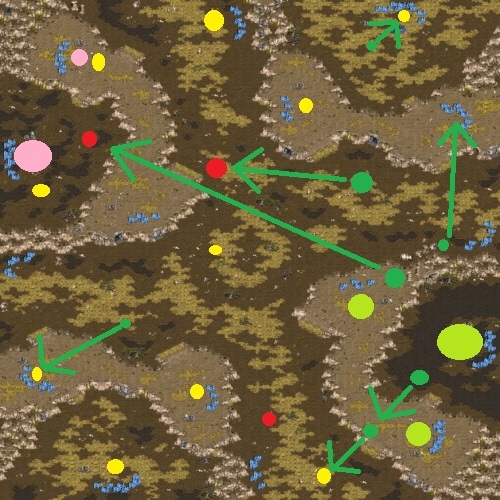
\includegraphics[scale=0.4]{mapassign5.jpg}
\caption{\label{fig:mapassign} A simple illustration of how units are assigned to tasks. Green dots are combat units owned by the bot, red dots are from the opponent. Light-green are bases of our bot, and pink are opponent's bases. Yellow dots are scout tasks for our bot. Green arrows indicate an assignment of a unit force on a task (red for combat or yellow for scout).}
\end{figure}

Notice that this approach is most likely not the best solution. In fact, it does not address the possibility that on the way to a task it may come across another task, which is possibly not appropriate at all for the unit. But on the other hand, the idea of tasks is merely to guide units to locations where we believe they can be put to maximum use. The unit itself can still decide to not pursue the received assignment.


\subsection{Forming Groups}
So far, we have considered assigning units to tasks separately. A problem that remained is how to actually assign units to tasks. Unfortunately, information on how many units of one type could handle an enemy force is not available. There are simply no pure statistics or quantitative information on this. This is important information, with which we could then allow our own units to divide themselves among different tasks instead of focusing on one specific task. 

We decided to make \emph{groups} of units, and assign groups to tasks instead of units to tasks. This makes sure that we can better allocate several units on the same task, with a better chance of completing it. Another reason for grouping is that this may make things computationally cheaper. For example, if there are 200 units on the battlefield and for each of the units we have to go through 50 lines of code before we decide an action per iteration of the program, the bot may become slower and slower. Therefore, if we consider a whole group of units, we essentially save time. 

Groups size was limited to 12 units, because the StarCraft engine only allows a maximum selection of 12 units at a time. Upon completion of a unit, it is assigned to one of the existing groups with which it has some similarities. For instance, a Hydralisk would be assigned to a group of other ranged units (Hydralisks and Lurkers). Another group would only consts of melee units such as Zerglings and Ultralisks. If there is no suitable group for a new unit, a new group is formed.

During battle, units can die, decreasing the number of units in a group. When a group's size drops under a certain threshold, the group is disbanded. The units are then reassigned to groups, allowing for indirect merging of groups.

\section{Micro}
\label{strategy:micro}
In this section we discuss the actual decision making of each unit. Using local information about a unit's surroundings and information about the general structure we have units make decisions individually. We describe our approach in general and mention several example rules, as well as a decision tree for one type of unit incorporating all the rules. Due to the enormous amount of rules (approx. 2000 lines), we do not show all of them.

The basic idea is to create \emph{emergent} behaviour by having each unit independently make decisions. This decision making is not very easy. As mentioned before there are many factors and it is not always very clear what decision is the best. To keep things simple, we extracted a number of simple rules on how units should behave. For example, rules such as "enemy in direct range and the number of nearby units is about as much units as the opponent have $\Rightarrow$ attack the nearest opponent", and "I am an Overlord (that can't attack), my goal is to observe something so I require to move there, but there are enemy turrets nearby $\Rightarrow$ move to a location that is outside the range of the enemy and is near my goal".

These kind of rules are not very difficult to obtain in general. For a human, it incorporates a lot of common sense ("avoid being damaged if I can't do harm"), and most of these kind of rules are also mentioned on websites or easily extracted from replay videos. For example, a psionic storm cast by a Protoss unit damages all units within the storm, so we order our units to move outside the storm. We saw this every time in replay videos, making it an important decision that overrules others. 

The difficulty lies in choosing the right order, or priority, of rules. We solved this by viewing the problem as a puzzle, where certain rules are obviously more important than others or apply more often in the general case. To keep decision making easy, we created decision trees for each type of unit, implicitly incorporating the rules that apply to them. In Figure \ref{fig:micro}, we illustrate the decision tree for units of the Zergling type as a flow chart.

\begin{figure}
\centering
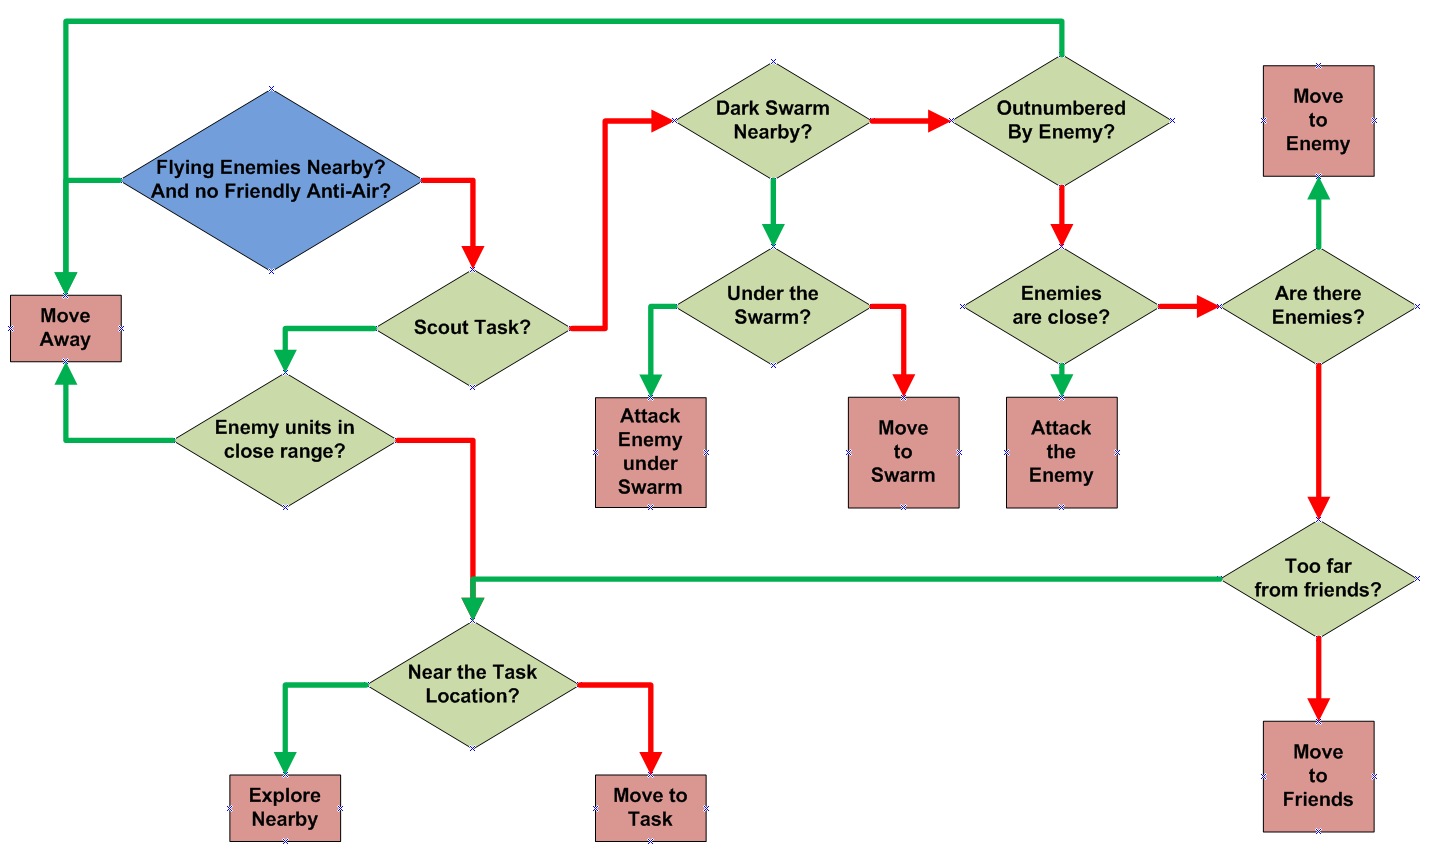
\includegraphics[scale=0.35]{starcraft_zerg_diagram_groot}
\label{fig:micro}
\caption{Flow chart illustration of the decision tree for Zergling units. The blue rhombus is the start and is a decision node. Green rhombi are also decision nodes. Red squares are decision terminals that are to be executed. Green lines indicate a 'yes' answer to the respective question, and red lines indicate 'no'.}
\end{figure}

We do not believe that our approach produces the best behaviour. In fact, because of the decision tree structure and our incomplete understanding of the game, it is very likely that certain decisions are not always appropriate. However, this is not the goal of the bot: instead we designed it to be capable of making decisions by itself, not only to initiate combat, but also to respond to the decisions of the opponent.

Units were allowed to make decisions using local information only, such as 'the number of enemy units within 12 steps from me'. Information about remote units is irrelevant for micro decisions, because actions by our units cannot affect those remote units, and vice versa. However if we only allow units to make decisions using local information, then it is unlikely that they will move elsewhere. To account for this, we designed the tasks and assignment plans, in section \ref{strategy:macro}. Basically, if there is 'nothing to do' for the unit on its current position, it will move to its assigned task's location. This is a low priority decision \emph{rule}, because we prioritize rules that directly affect the unit's state. As a result, we can have units move towards a task, and if it finds enemy units nearby, it will move away or engage in combat.

During the concept and implementation phases, micro took the most time to complete. There were many cases where we coded our units to behave in a certain way, only to find out that they did not do what they were supposed to. In some cases, we even found that decision rules caused a deadlock between the units. The most interesting one was a conflict with the worker unit, the Drone: the rules "if there are five drones on minerals and no drone gathers vespene gas $\Rightarrow$ go to gas", and "if we have few minerals, a few drones on gathering minerals, and I am gathering vespene gas $\Rightarrow$ go gather minerals instead". As a result of these rules, none of the nearby drones were actually doing anything. This is because at every iteration of the program (of which there are around 25 per second), units make the decisions to gather minerals; the next iteration one unit goes for gas; then the next iteration it goes back to minerals; then another unit goes for gas; and so on. Because of small delays in executing decisions, units did move very slowly to minerals, but never accomplished to gather any as they weret interrupted several times per second.

Another problem of our initial implementation is that decision making could become too computationaly intensive as we trained more units. This is because many of the decision rules included many checks on whether there are enemy units nearby, which was programmed to enumerate every known enemy and check their location. One idea to solve this was to memorize the nearby units we checked. However, this caused our units to not respond fast to new situations as it may think the units were still there, when they in fact were not.

Another solution that we thought of, was \emph{copying} a decision made by one unit to other nearby units that are the same type of unit. We believe this was a good idea as we avoid computing the same for nearby units, for which it is very likely that the same conditions apply. This solution also makes units more likely to work together. By controlling the range of nearby units we avoid cases where far distant units do the same. This is also why we did not have a whole group make a single decision. We experimented with this idea of decision making over groups for Zerglings and Mutalisks (two types of units that tend to flock), but found often that some of the units were too far away from each other, making group decisions often inappropriate for units individually.







%Don't forget to devote part of your report to your motivation for your game. What is special (unique) about your game, is it commercially interesting or technologically innovative? That kind of stuff. *************************************************************************



%
%, where it tries to simulate the aftereffects of decisions. For example in a game of Chess, the computer can easily simulate what will happen when it moves its pieces. Then by evaluating the simulated state of the game we get insight in how 'good' a certain move is. If we do this many times, we then can pick the action that is the best in general. This approach, however, assumes that we know how moving pieces change the board. And it assumes that we can rely on our evaluation of the simulated board as a good indication of how good a decision is.
%
%Another type of technique is to 'learn' how to play. This approach attempts to learn the consequence of a decision. This implicitly includes both how to simulate the board, and the evaluation of the board (or rather the 'goodness' of a decision). Unfortunatey, learning is often a very hard task to do. In addition it may cost a lot of time. The major reason for this is that the 'learning'-algorithms are either very general or intrinsically limit the capabilities of learning somehow (e.g. a 'bias'). Although there are possibilities to include domain knowledge, they are not for every type of problem easy to come by.
%
%The same holds for the game of StarCraft. Although there is plently of information on what a structure or unit is capable of, the interplay and dynamics between multiple diverse units makes it complex to understand how everything works.
%
%In theory, we believe it is feasible to simulate complete boards. The trouble is that it the number of boards easily exploits to massive numbers. For instance, each combat unit can do 4 to 10 different actions, such as moving, attacking and abilities.\footnote{Some of the abilities can be cast in a whole nearby area of the unit, making the number of possible actions even bigger. For now, we take actions in general for simplicity.} During the game, we have any number between 12 to 500 units. The number 12 is how every game is started (each player 5 worker units and a main building). Although very high numbers such as 500 are rare, they are still possible in the game. For now, we estimate an average of 150 units per game, which have on an estimated average of 6 different actions. This results in $6^150$ possible different boards already. And this is only one step deep of simulation, i.e. 1 ply. It is easy to see that this number is excessively large and that simulating games of several ply deep is computationally intractable.
%
%As for learning, we have to deal with challenges of the same complexity. Even if we assume that we can completely simulate boards, we still have the problem of learning to associate decisions with boards. 
%
%



%Research in the field of Artificial Intelligence have shown that there are ways for a computer (that 'plays' the bot) to learn the consequences of its actions. Most often these are techniques related to 'Machine Learning', such as supervised learning or reinforcement learning.
%
%An alternative to 
%
%Depending on the input from the game or its own inner variables, it makes decisions. 
%
%Obviously, if a bot makes a decision it has certain consequences for the game. The hard part is to make good decisions that have consequences that are benefiicial to the cause of the bot (i.e. winning, or creating interesting gameplay for the person playing the game). For example, if it recklessly sends small armies to the player that it can easily beat does not make the game very interesting. Or when it creates units that can only take air units, while the player made no air units. 
%
%
%The 'artificial intelligence' of bots in games is usually just constructed with some simple scripts. 
%
%\begin{enumerate}
%	\item Predictable, they always choose the same action in same cases.
%	\item Non-reactive, no matter what the player does, the bot will just do its own thing
%
%
%\end{enumerate}
%
%
%A common problem for bots is that they tend to be predictable. This is most often because they follow a simple deterministic script. For example, it always makes the same buildings in the same order. Or it creates repetitive behaviour, such as repeating 'create 10 units, send them to the player' over and over.
%
%
%
% 10 units, send them to the enemy, and then starts over again. This makes the bot's decisions rather predictable. 
%
%
%
